\documentclass[twocolumn, 10pt]{article}
\usepackage{graphicx}
\usepackage{amsmath, bm}
\usepackage{wrapfig}
\usepackage{natbib}
\usepackage{tikz}
\usepackage{amssymb}
\usepackage{caption}
\usepackage{amstext}
\usepackage[greek,english]{babel}
\usepackage{amsmath}
\usepackage[utf8]{inputenc}
\usepackage{fancyhdr}
\usepackage{caption}
\usepackage[margin=0.6in]{geometry}
\hyphenpenalty=10000
\captionsetup[figure]{font=footnotesize}
\newcommand{\changefont}{\fontsize{9}{10}\selectfont}
\pagestyle{fancy}
\fancyhf{}
\rhead[LE,RO]{\changefont \slshape Literature Review}
\lhead[RE,LO]{\changefont \slshape The Search for Magnetic Monopoles}
\cfoot{\thepage}
\renewcommand{\headrulewidth}{2pt}
\renewcommand{\footrulewidth}{1pt}
\begin{document}
\captionsetup[figure]{labelfont={bf},name={Fig.},labelsep=period}
\title{\textbf{The Search for Magnetic Monopoles}}
\author{James Ovenden}
\date{\today}
\maketitle

\tableofcontents

\section{Introduction}
Emmy Noether showed us that nature and symmetry are intrinsically linked on the physical level using Lagrangian mechanics. She theorised that for a particular symmetry in a particle's Lagrangian, there is an associated conserved quantity \cite{bob2017purdy}. Noether's theorem is considered by many to be one of the most beautiful results of mathematics and \textit{`a guiding star to 20th and 21st century physics'} according to Professor Frank Wilczek of MIT \cite{scinews}. It is the human condition to continue to search for such satisfying and beautiful phenomena in the Universe and this elegance in physics doesn't end there; another such example comes in the form of Maxwell's equations. \\
\indent James Clerk Maxwell formulated his equations in 1861 and developed the symmetry between electricity and magnetism \cite{maxwell1861li}. It can be easily seen, even with the presence of arbitrary constants, that both the electric and magnetic fields are almost indistinguishable in the absence of a source 
\begin{equation*}
\nabla \cdotp \mathbf{E} = 0   \ \ \text{(1.1a)} \ \ \ \ \ \ \  \nabla \times \mathbf{E} = \frac{-1}{c}\frac{\partial \mathbf{B}}{\partial t} \ \  \text{(1.3a)}
\end{equation*}
\begin{equation*}
\ \ \ \ \ \ \ \ \ \ \ \ \ \nabla \cdotp \mathbf{B} = 0   \ \ \text{(1.2a)} \ \ \ \ \ \ \ \ \ \ \ \nabla \times \mathbf{B} = \frac{1}{c} \frac{\partial \mathbf{E}}{\partial t} \ \ \text{(1.4a)} \ \ \ \ \ \ \ \ \ \ \ \ \ \ \ \ \ \ \ 
\end{equation*} 
where Gaussian unit convention is used. Introducing an electric charge and current into the system, the equations become \cite{maxwell1861li, martin2015phys}
\begin{equation*}
\nabla \cdotp \mathbf{E} = 4\pi\rho  \ \ \text{(1.1b)} \ \ \ \ \ \ \  \nabla \times \mathbf{E} = \frac{-1}{c}\frac{\partial \mathbf{B}}{\partial t} \ \  \text{(1.3b)}
\end{equation*}
\begin{equation*}
\ \ \nabla \cdotp \mathbf{B} = 0   \ \ \text{(1.2b)} \ \ \ \ \ \ \ \ \ \ \ \ \ \ \ \ \nabla \ \times \ \mathbf{B} = \frac{1}{c}\left(4\pi\mathbf{J} + \frac{\partial \mathbf{E}}{\partial t}\right) \ \ \text{(1.4b)}\text{.} \ \ \ \ \ \ \ \ \ \ \ \ \ \ \ \ \ \ \      
\end{equation*}
Though still beautiful, this offers an unsatisfying result. The symmetry between $\mathbf{E}$ and $\mathbf{B}$ is lost. So far, though, only an electric point charge is present in the system. Let's see what happens when a magnetic point source is introduced. This gives Maxwell's equations in the form \cite{ellismagnetic}
\begin{equation*}
\ \ \ \ \ \ \nabla \cdotp \mathbf{E} = 4\pi\rho  \ \ \text{(1.1c)}  \ \ \ \ \ \ \ \ \ \ \ \   \nabla \times \mathbf{E} = \frac{-1}{c}\left(\frac{\partial \mathbf{B}}{\partial t} + 4\pi\mathbf{J}_{m}\right) \ \  \text{(1.3c)}
\end{equation*}
\begin{equation*}
\ \ \ \ \ \ \nabla \cdotp \mathbf{B} = 4\pi\rho_{m}  \ \ \text{(1.2c)} \ \ \ \ \ \ \ \ \ \ \ \ \nabla \times \mathbf{B} = \frac{1}{c}\left(4\pi\mathbf{J} + \frac{\partial \mathbf{E}}{\partial t}\right) \ \ \text{(1.4c)} \ \ \ \ \ \ \ \ \ \ \ \ \ \ \ \ \ \ \      
\end{equation*}
with $\rho_{m}$ and $\mathbf{J}_{m}$ being magnetic charge density and current respectively. The symmetry has been restored! This magnetic monopole provides a wonderful solution to this symmetry `problem'. We've yet to observe such a particle but this doesn't mean that it isn't present in nature, as Paul Dirac once wrote---\textit{`one would be surprised if nature made no use of it'} \cite{dirac1931quantised}. \\
\indent The magnetic monopole is and has been the subject of many a physicist's entire career. Its discovery would help us paint the mathematical picture of the Universe we live in due to its prevalence in Grand Unified Theories, it would give us a fundamental reason for the quantisation of electric charge and help to confirm one of the most radical, but now widely accepted, concepts in cosmology. This short paper aims to look at the reasons we believe this particle exists, its elusiveness, and the impact it has had on the theories predicting its existence. 

\section{Electric Charge Quantisation}

Philosophical physicists might posit the question of why the Universe possesses the particular characteristics we observe. This is a question that we may never be able to answer fully; we could be seeing most phenomena in the Universe merely because that is how our universe behaves (we also can't compare to any others!). The quantisation of electric charge in the form of the electron might have been considered by many to be of such nature, but it was Paul Dirac who was able to prove why using the existence of a magnetic point source. \\
\indent The charge quantisation condition can be proven using T.T. Wu's and C.N. Yang's approach who constructed a theory of the Abelian monopole in 1975 \cite{WuMonopoleYang}, but first a revisit Dirac's 1931 paper is required. Dirac postulated the idea of a string, analogous to an infinitely thin solenoid, that ended with a monopole. They are unobservable and lead to an unpleasant proof but can be eliminated using the Wu-Yang monopole method.  The concept of two overlapping hemispheres with identical radii, $\mathbf{R^n}$ and $\mathbf{R^s}$, is used in a magnetic monopole (isotropic) field contained within $\mathbb{R}^3$ space. Being a non-singular theory, one must remove the monopole---as it is, itself, a singularity---from the origin. So, therefore, only consider the $\mathbb{R}^3$/\{$0$\} space.\\
\begin{figure}[t]
\centering
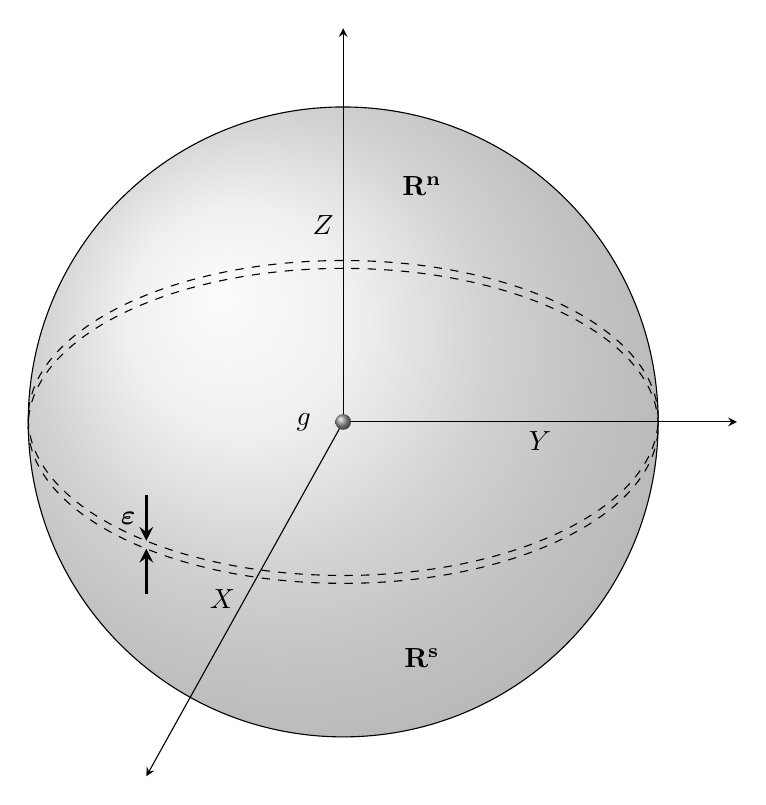
\begin{tikzpicture}
\shade[ball color = gray!40, opacity = 0.4] (0,0) circle (4cm);
\draw (0,0) circle (4cm);
\draw[dashed] (4,0.05) arc (0:360:4 and 2);
\draw[dashed] (4,-0.05) arc (0:360:4 and 2);
\fill[fill=black] (0,0) circle (1pt);
\draw[ ->, >=stealth] (0,0 ) -- node[below]{$Y$} (5,0);
\draw[ ->, >=stealth] (0,0 ) -- node[left]{$Z$} (0,5);
\draw[ ->, >=stealth] (0,0 ) -- node[left]{$X$} (-2.5,-4.5);
\draw[very thick, ->, >=stealth] (-2.5,-0.93) -- node[left]{$\bm{\varepsilon}$} (-2.5,-1.51);
\node (a) at (1,3) {$\mathbf{R^n}$};
\node (b) at (1,-3) {$\mathbf{R^s}$};
\node (c) at (-0.5,0) {$g$};
\draw[very thick, ->, >=stealth] (-2.5,-2.19) -- node[left]{$$} (-2.5,-1.61);
\shade[ball color = black!40] (0,0) circle (0.1cm);
\end{tikzpicture}
\caption{Two overlapping hemispheres, $\mathbf{R^n}$ and $\mathbf{R^s}$, in $\mathbb{R}^3$. Removing singularity $g$ would give this arrangement in the $\mathbb{R}^3$/\{$0$\} space.}
\end{figure}

\indent One can define potentials in these regions

\begin{equation} \tag{2}
\mathbf{A^n} = g\frac{1 - \cos\theta}{r\sin\theta}\hat\phi \ \ \ \ \ \ \ \ 0 \leq \theta < \frac{\pi}{2} + \frac{\bm{\varepsilon}}{2}
\end{equation}
\begin{equation}\
\mathbf{A^s} = -g\frac{1 + \cos\theta}{r\sin\theta}\hat\phi \ \ \ \ \ \ \ \ \frac{\pi}{2} - \frac{\bm{\varepsilon}}{2} < \theta \leq 0
\end{equation}
where $g$ is the magnetic charge and $r$ the radius of the hemispheres. With the string lying along the $z$-axis, the coordinate system has been defined such that it no longer needs to be considered. The limits on $\theta$ that allow the string to be excluded are $\theta = \pi$ in $\mathbf{A^n}$ and $\theta = 0$ in $\mathbf{A^s}$. Now no singularities exist in the system. \\
\indent It can be seen from Fig.~1. that the area of overlap, $\bm{\varepsilon}$, is infinitesimal and is equal to $\mathbf{R^n}\cap\mathbf{R^s}$. Although these hemispheres contain two different potentials,  they encompass the same magnetic field. Using this fact and equation 1.2c it can be shown that $\mathbf{B} = \nabla\times\mathbf{A^n} = \nabla\times\mathbf{A^s}$. It follows that $\mathbf{A^n}$ and $\mathbf{A^s}$ are related with a gauge transformation in $\bm{\varepsilon}$. As previously mentioned, $\bm{\varepsilon}=\mathbf{R^n}\cap\mathbf{R^s}$. Thus the limits of $\theta$ for this region can be defined: $\frac{\pi}{2} - \frac{\bm{\varepsilon}}{2} < \theta < \frac{\pi}{2} + \frac{\bm{\varepsilon}}{2}$. Now a gauge function can be deduced using the difference in these potentials. It can be seen from equations 2 and 3 that in region $\bm{\varepsilon}$, 

\begin{equation}
\mathbf{R^n}-\mathbf{R^s}=\frac{2g\hat\phi}{r\sin\theta}=\frac{2g\hat\phi}{r\sin(\frac{\pi}{2}\pm\frac{\bm{\varepsilon}}{2})}=\frac{2g\hat\phi}{r}
\end{equation}

as $\bm{\varepsilon}\longrightarrow0$, and thus

\begin{equation}
\frac{2g\hat\phi}{r} = \nabla(2g\phi) = \nabla\bm{\Lambda}
\end{equation}
where $\bm{\Lambda}$ is a newly defined gauge function: $\bm{\Lambda} = 2g\phi$.\\
\indent It is at this point where an electric point charge is introduced, two wavefunctions are required here $\bm{\psi}^n$ in $\bm{R}^n$ and $\bm{\psi}^s$ in $\bm{R}^s$. If this charge lies within the region $\bm{\varepsilon}$, the aforementioned wavefunctions must be related by a phase transformation of the form

\begin{equation}
\bm{\psi}^n = \bm{e}^\frac{iq\bm{\Lambda}}{\hbar c}\bm{\psi}^s = \bm{e}^\frac{iq\bm{2g\phi}}{\hbar c}\bm{\psi}^s.
\end{equation}
A wavefunction can only have one value at a single point, so allowing the electric charge to traverse $2\pi$ around the sphere within $\bm{\varepsilon}$ (for the sake of simplicity, in the $x-y$ plane) will yield the same value. This leads to the case that $\bm{\psi}^n|_\phi = \bm{\psi}^n|_{\phi+2\pi}$. It can now be deduced that 

\begin{equation}
\bm{\psi}^n = \bm{e}^\frac{iq\bm{2g\phi}}{\hbar c}\bm{\psi}^s = \bm{e}^\frac{iq\bm{2g(\phi+2\pi)}}{\hbar c}\bm{\psi}^s
\end{equation}
and so

\begin{equation}
\bm{e}^\frac{iq\bm{2g\phi}}{\hbar c} = \bm{e}^\frac{iq\bm{2g(\phi+2\pi)}}{\hbar c}
\end{equation}
which leads to

\begin{equation}
\bm{e}^\frac{iq\bm{g4\pi}}{\hbar c} = 1.
\end{equation}
From this, it is now clear that 

\begin{equation}\
qg = \frac{n\hbar c}{2}.
\end{equation}
\\
\indent This wonderfully elegant proof shows that the presence of the magnetic monopole would give a reason for the quantised nature of electric charge and, as such, a huge reason to speculate their existence \cite{Heras_2018, shnir, preskill1984magnetic}.

\section{Magnetic Monopoles in Cosmology}
It turns out that the concept of the magnetic monopole plays a large part in our understanding of how the Universe behaved in its very early stages. A now widely accepted theory of the Universe's inception used the idea of inflation and was presented by Alan Guth in 1981 \cite{liddle2015cosmo, guth1981inflate}, but it was another of his papers published a year prior that explored the importance of the magnetic monopole.

\subsection{Monopole Production in the Early Universe}
\subsubsection{Higgs Field Symmetry Breaking}
The early Universe is thought to have been incredibly hot but it was also cooling at a rapid rate. Eventually, the temperature would be such that spontaneous symmetry breaking could occur in the Higgs field, at around $10^{15}$ GeV. Guth proposed the idea of entities called `bubbles', these would develop from a phase transition at a single point with a particular value in the Higgs field. A bubble greater than a critical size would expand as it would be energetically favourable for surrounding areas of the field to fall into the same configuration, giving them the same value. One can visualise this as being analogous to a growing crystalline structure.

\begin{figure}[h]
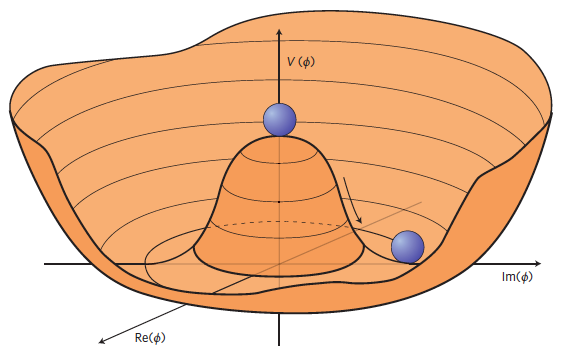
\includegraphics[width=\linewidth]{higgspotential.png}
\caption{`Mexican hat' Higgs potential. One can see that values in the field are determined randomly when symmetry is broken \cite{Ellis_2016}.}
\end{figure}
\subsubsection{From Bubbles to Monopoles}
Bubbles could lead to the production of a monopole in different ways, but the easiest to visualise and the first presented by Guth was the idea of `bubble coalescence'. This would involve two separate bubbles, both initially out of causal contact with each other, growing and eventually coming into contact. These bubbles would most likely have different values in the Higgs field, and so to extrapolate on the crystal analogy: they would have differing orientations. The field would then attempt to align itself, conserving as much energy as possible between these different orientations, and the result is a topological defect or \textit{knot}. This knot would be a magnetic monopole \cite{guth1980early}.

\begin{figure}[h]
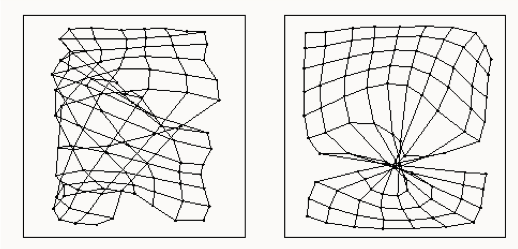
\includegraphics[width=\linewidth]{Topological_defect.png}
\caption{`Topological defects of a two-dimensional network: left folding, right twist' - Visualisation of a knot in the Higgs field \cite{topological2005defect}.}
\end{figure}

\subsection{The Magnetic Conclusion}
One might have taken for granted that this `defect' in the Higgs field is a magnetic monopole, but it can be proven that this is of magnetic nature. Consider a sphere of radius $\bm{r}$ with the defect at the centre, the potential energy associated with the Higgs field $\mathbf{H}$ within this sphere is

\begin{equation}
\mathbf{E}_{Higgs} = 4\pi \int (\nabla\mathbf{H})^2 \bm{r}^2 d\bm{r}.
\end{equation}
When in close proximity to the defect, calculating $\nabla\mathbf{H}$ can be quite complicated. Far away, though, the gradient of the Higgs field varies with the inverse of the radius. This gives an integral of the form

\begin{equation}
\mathbf{E}_{Higgs} = 4\pi \int \left(\frac{1}{\bm{r}}\right)^2 \bm{r}^2 d\bm{r} = 4\pi\bm{r}.
\end{equation}

As previously mentioned, the defect is a 0-dimensional singularity. A point in spacetime (and thus, in the Higgs field). One could, therefore, be forgiven for questioning this result, which suggests that the energy diverges with the radius of the sphere. The answer comes when taking coupling between fields into consideration; this example only considers energy in the Higgs field, but there is also strong coupling to vector boson fields. When the calculation is redone using this fact, it is found that the divergence from the integral disappears and it also introduces the necessary magnetic terms. \cite{guth2015lecs}

\subsection{The Magnetic Monopole Problem}

The Magnetic Monopole Problem takes the idea of symmetry breaking in the early Universe further. With the temperatures lowering, it is statistically likely that many regions of the Higgs field will eventually have their symmetry broken. Thomas Kibble showed that one can assume 1 monopole per causally connected region of the Higgs field \cite{kolb1990early, arrtu2013conf}. This allows for calculation of the monopole number density. 

\subsubsection{Kibble's Formalism}
The minimum distance at which two areas are out of causal contact with each other is defined to be $\zeta$. There is also a probability $\bm{p}_{monopole}$ associated with production of a monopole which also takes into account monopole-antimonopole annihilation, but as previously mentioned this value will be very close to 1. This gives a monopole density in the phase transition of \cite{preskill1984magnetic}

\begin{equation}
\bm{n}_{monopole} = \frac{\bm{p}_{monopole}}{\zeta^{3}}.
\end{equation}

It is difficult to compute an exact value for $\zeta$ but, using the concept of the particle horizon, it can be narrowed down. The particle horizon will be the shortest distance that is out of causal contact with an observer, so this must be the upper bound

\begin{equation}
\zeta < \bm{r}_H.
\end{equation}
This also gives a lower bound on the monopole density

\begin{equation}
\bm{n}_{monopole} = \frac{\bm{p}_{monopole}}{\bm{r}_H^3}.
\end{equation}
\subsubsection{Scale Factor, Density and Time due to Monopoles}
GUT symmetry breaking is believed to have occurred at $t_{GUT}\approx10^{-36}$s. Taking this to be the moment of creation for all monopoles, it is found that

\begin{equation}
\bm{n}_{monopole,t_{GUT}} = \frac{\bm{p}_{monopole}}{(2ct_{GUT})^3} \approx 10^{81}.
\end{equation}
To calculate the ratio of the Universe's scale factor, $\bm{a}$, between $t_{GUT}$ and now, consider that $\rho_{radiation} \propto \bm{a}^{-4}$. Treating the Universe as a perfect blackbody, this gives the result $T \propto \bm{a}^{-1}$ and yields a value for $\bm{a}$ of the form \cite{liddle2015cosmo}

\begin{equation}
\bm{a}_{t_{GUT}} = \frac{T_{CMB}}{T_{GUT}} = \frac{T_{CMB}k_B}{10^{15}GeV} \approx 10^{-29}.
\end{equation}

Matter varies as $\rho_{mat} \propto \bm{a}^{-3}$, this would result in a current monopole density of

\begin{equation}
\bm{n}_{m,t_{0}} = \frac{\bm{n}_{m,t_{GUT}}}{{\bm{a}_{t_{GUT}}^3}}= \frac{10^{82}}{(10^{-29})^{-3}} \approx 1 \text{ monopole } m^{-3}
\end{equation}
where $\bm{n}_{m,t_{0}} = \bm{n}_{monopole,t_{now}}$. The mass of a magnetic monopole turns out to be approximately $\frac{1}{\alpha}\times$the scale of GUT symmetry breaking where $\alpha$ is the fine structure constant of electrodynamics ($\approx\frac{1}{137}$) \cite{guth2015lecs}. This gives the monopole a staggering mass of around $10^{17}$ GeV$c^{-2}$ or $0.2 \mu g$! Mass density due to monopoles is thus found to be $\bm{\rho}_m = 0.2\times10^{-9} kgm^{-3}$, as such this value can be used to calculate the age of the Universe merely due to magnetic monopoles. One can start with the density parameter $\Omega(t)$ \cite{liddle2015cosmo}---

\begin{equation}
\Omega(t) = \frac{\bm{\rho}_m}{\bm{\rho}_c}
\end{equation}
where $\bm{\rho}_c$ is the critical density of the Universe. The equation \cite{guth2015lecs}

\begin{equation}
t = \frac{\pi}{2H\sqrt\Omega}
\end{equation}
gives an upper bound on time of 206 years. After careful consideration, one might suggest that this is, in fact, not the age of the Universe. This is the crux of the Magnetic Monopole Problem, and it gave way to one of the most radical ideas in cosmology. \\
\indent Alan Guth proposed that this problem could be nullified if the early Universe underwent a period of rapid inflation, whereby 1$m^3$ of the Universe pre-inflation would increase to around $10^{43}m$ in around $10^{-34}$s, or to about the size of the observable Universe! This `inflated' away the monopoles \cite{rajantie2012magnetic, liddle2015cosmo} along with any other `relic particles' and would suggest that there may be only a single monopole in our region of the cosmos from its inception.

\section{Conclusion}

Unfortunately, only magnetic monopole-like objects have been observed: as quasi-particles in condensed matter \cite{ray2015observation}, real monopoles have never been directly observed in nature. It is a testament to the beauty of the concept and the ideas presented that so much of Theoretical and Experimental Physics has been dedicated to it. This is true in both theorising its characteristics and in methods for its potential discovery. Research facilities such as MoEDAL in the LHC and cosmic ray observatories on the South Pole currently lead the way in finding such phenomena and are not the first to have attempted to do so \cite{rajantie2012introduction}. \\
\indent Many theorists suggest that we can be sure of their existence even without observation, that \textit{`the existence of magnetic monopoles seems like one of the safest bets that one can make about physics not yet seen'} \cite{Polchinski_2004}. But for now, in spite of such concrete theory, the lack of observation means the search must continue. Such lack of discovery does not change the important results provided to Grand Unified Theories, Cosmology and Electromagnetism along with the further insight given into high energy Theoretical Physics. As such, magnetic monopoles are integral to our description of the Universe, whether they exist or not.

\bibliographystyle{unsrt}
\bibliography{LitRevRefs.bib}
\end{document}